\documentclass[11pt,a4paper]{article}

% ==============================================================================
% PACOTES ESSENCIAIS E CONFIGURAÇÕES DE IDIOMA E FONTE
% ==============================================================================
\usepackage[utf8]{inputenc}
\usepackage[T1]{fontenc}
\usepackage[portuguese]{babel}
\usepackage{lmodern}
\usepackage{microtype}
\setlength{\emergencystretch}{3em}

% Geometria da página
\usepackage[a4paper, top=2.5cm, bottom=2.5cm, left=2.5cm, right=2.5cm]{geometry}

% Matemática e símbolos
\usepackage{amsmath, amssymb}

% Imagens, figuras e tabelas
\usepackage{graphicx}
\usepackage{booktabs}
\usepackage{array}
\usepackage{float}
\usepackage{needspace}
\usepackage{enumitem}

% Cores e caixas de destaque
\usepackage[dvipsnames,svgnames,x11names]{xcolor}
\usepackage[many]{tcolorbox}

% Código QR para o vídeo
\usepackage{qrcode}

% Cabeçalhos e rodapés
\usepackage{fancyhdr}
\pagestyle{fancy}
\fancyhf{}
\fancyhead[L]{\small\textbf{Integração de Sistemas de Informação} -- Trabalho Prático I}
\fancyhead[R]{\small\thepage}
\fancyfoot[L]{\small IPCA -- Licenciatura em Engenharia de Sistemas Informáticos}
\fancyfoot[R]{\small Pentaho Kettle}
\renewcommand{\headrulewidth}{0.6pt}
\renewcommand{\footrulewidth}{0.4pt}
\setlength{\headheight}{14pt}

% Hiperligações
\usepackage{hyperref}
\hypersetup{
    colorlinks=true,
    linkcolor=NavyBlue,
    citecolor=OliveGreen,
    urlcolor=RoyalBlue,
    pdftitle={TP1-ISI: Há campo? Integração da disponibilidade de campos de ténis},
    pdfauthor={Alexandre Machado (31499)}
}
\urlstyle{tt}
\addto\captionsportuguese{\renewcommand{\contentsname}{Conteúdo}}

% Listagens (SQL, JavaScript, comandos)
\usepackage{listings}
\usepackage{textcomp}
\renewcommand{\lstlistingname}{Listagem}
\definecolor{codegreen}{rgb}{0.13,0.55,0.13}
\definecolor{codeblue}{rgb}{0.0,0.3,0.7}
\definecolor{codepurple}{rgb}{0.58,0,0.82}
\definecolor{backcolour}{rgb}{0.96,0.96,0.96}
\lstdefinestyle{tpstyle}{
    backgroundcolor=\color{backcolour},
    commentstyle=\color{codegreen},
    keywordstyle=\color{codeblue},
    stringstyle=\color{codepurple},
    basicstyle=\ttfamily\scriptsize,
    upquote=true,
    breaklines=true,
    captionpos=b,
    keepspaces=true,
    numbers=none,
    xleftmargin=4pt,
    framexleftmargin=4pt,
    showstringspaces=false,
    columns=fullflexible,
    frame=single,
    rulecolor=\color{black!15},
    literate={á}{{\'a}}1 {à}{{\`a}}1 {â}{{\^a}}1 {ã}{{\~a}}1
             {é}{{\'e}}1 {ê}{{\^e}}1 {í}{{\'i}}1
             {ó}{{\'o}}1 {ô}{{\^o}}1 {õ}{{\~o}}1 {ú}{{\'u}}1
             {ç}{{\c{c}}}1 {Á}{{\'A}}1 {É}{{\'E}}1 {Ç}{{\c{C}}}1
             {º}{{\textordmasculine}}1
}
\lstset{style=tpstyle}

% Caixa para a ligação do vídeo (mesmo formato das fichas de SETR)
\newtcolorbox{videoBox}[1]{
    colback=NavyBlue!3!white,
    colframe=NavyBlue!75!black,
    fonttitle=\bfseries\small,
    title=#1,
    arc=2mm,
    boxrule=0.6pt,
    left=2mm, right=2mm, top=1mm, bottom=1mm
}

% ==============================================================================
% DADOS DE IDENTIFICAÇÃO
% ==============================================================================
% O ficheiro submetido deve ser: <número de aluno>_doc.pdf  ->  31499_doc.pdf
\newcommand{\anoLetivo}{2026/2027}
\newcommand{\alunoNome}{Alexandre Magalhães Martins Machado}
\newcommand{\alunoNum}{31499}
\newcommand{\docente}{Óscar Ribeiro}
\newcommand{\dataEntrega}{22 de outubro de 2026}

% Ligação do vídeo de demonstração (deixar vazio enquanto não existir)
\newcommand{\videoURL}{}

% ==============================================================================
% DOCUMENTO
% ==============================================================================
\begin{document}

% ------------------------------------------------------------------------------
% CAPA
% ------------------------------------------------------------------------------
\begin{titlepage}
    \centering
    \vspace*{0.5cm}

    {\scshape\Large Instituto Politécnico do Cávado e do Ave\par}
    {\scshape\large Escola Superior de Tecnologia\par}
    \vspace{0.3cm}
    {\large Unidade Curricular: \textbf{Integração de Sistemas de Informação (ISI)}\par}

    \vspace{1.8cm}
    \hrule height 1.5pt
    \vspace{0.4cm}
    {\huge\bfseries Relatório do Trabalho Prático I\par}
    \vspace{0.3cm}
    {\LARGE Há campo?\par}
    \vspace{0.2cm}
    {\large\textit{Integração da disponibilidade de campos de ténis de vários clubes\\com Pentaho Data Integration (Kettle) e PostgreSQL}\par}
    \vspace{0.4cm}
    \hrule height 1.5pt
    \vspace{1.5cm}

    \begin{tcolorbox}[colback=gray!5!white,colframe=gray!50!black,arc=2mm,title=\textbf{Identificação}]
        \centering
        \begin{tabular}{ll}
            \textbf{Aluno:} & \alunoNome{} (N.º \alunoNum) \\
            \textbf{Curso:} & Licenciatura em Engenharia de Sistemas Informáticos (pós-laboral) \\
            \textbf{Docente:} & \docente \\
            \textbf{Modalidade:} & Trabalho individual \\
        \end{tabular}
    \end{tcolorbox}

    \vfill

    {\large Ano Letivo: \textbf{\anoLetivo}\par}
    \vspace{0.5cm}
    {\small Barcelos, \dataEntrega\par}
\end{titlepage}

% ------------------------------------------------------------------------------
% ÍNDICE
% ------------------------------------------------------------------------------
\tableofcontents
\newpage

% ------------------------------------------------------------------------------
% 1. ENQUADRAMENTO
% ------------------------------------------------------------------------------
\section{Enquadramento}

\begin{table}[H]
\centering
\caption{Identificação do trabalho.}
\label{tab:identificacao}
\renewcommand{\arraystretch}{1.2}
\begin{tabular}{@{}p{3.4cm}p{11.4cm}@{}}
\toprule
\textbf{Equipa} & \alunoNome{} (\alunoNum), trabalho individual \\
\textbf{Unidade curricular} & Integração de Sistemas de Informação, 3.º ano, 1.º semestre, \anoLetivo \\
\textbf{Curso} & Licenciatura em Engenharia de Sistemas Informáticos, regime pós-laboral, IPCA \\
\textbf{Plataformas} & Pentaho Data Integration (Kettle) 10.2, PostgreSQL 17, API REST Open-Meteo; página HTML/JavaScript para apresentar o resultado \\
\bottomrule
\end{tabular}
\end{table}

O enunciado do Trabalho Prático I~\cite{enunciado} pede o desenvolvimento de um processo ETL (\textit{Extract, Transform, Load}) completo, com dados de várias origens e formatos, transformações de limpeza e de lógica de negócio e vários destinos. O tema parte de um projeto pessoal, o \textbf{hacampo} (\textit{``Há campo?''}): um quadro público que mostra a qualquer jogador que campos de ténis estão livres ou ocupados num clube, sem ser necessário telefonar.

% ------------------------------------------------------------------------------
% 2. PROBLEMA
% ------------------------------------------------------------------------------
\section{Problema}

Em muitos clubes de ténis não é possível consultar online se há campos livres. As marcações estão repartidas por sistemas que não comunicam entre si: num clube são escritas num caderno no bar e passadas para Excel; noutro existe uma aplicação apenas para sócios; num complexo municipal estão na agenda da câmara. Quem quer jogar tem de contactar cada um.

O objetivo do trabalho é \textbf{integrar as marcações de três clubes num único quadro de disponibilidade}. Para isso é necessário resolver problemas típicos de integração ao nível dos dados, resumidos na Tabela~\ref{tab:problemas}.

\begin{table}[H]
\centering
\caption{Problemas de integração encontrados nos dados.}
\label{tab:problemas}
\small
\renewcommand{\arraystretch}{1.25}
\begin{tabular}{@{}p{4.2cm}p{10.6cm}@{}}
\toprule
\textbf{Problema} & \textbf{Exemplo nos dados} \\
\midrule
Formatos diferentes & CSV com \texttt{;}, JSON com objetos aninhados, XML com atributos e validação por XSD \\
O mesmo valor escrito de várias formas & datas \texttt{21/10/2026}, \texttt{2026-10-21}, \texttt{21-10-26}; horas \texttt{18h}, \texttt{18:00}, \texttt{18.30}, \texttt{18H}; campos \texttt{C1}, \texttt{Campo 1}, \texttt{court 1}; telefones \texttt{+351 912\ldots}, \texttt{00351912\ldots} \\
Dados incompletos ou inválidos & reserva sem hora, data sem ano, campo que não existe, reserva depois do fecho do clube \\
Registos repetidos & linha escrita duas vezes no caderno; a aplicação envia a mesma reserva duas vezes (mesmo \texttt{id}); reservas canceladas \\
Dados pessoais & nomes, telefones e emails não podem aparecer num quadro público (RGPD~\cite{rgpd}) \\
Informação de outros sistemas & se vai chover num campo descoberto e se já é de noite num campo sem iluminação \\
Conflitos de negócio & duas reservas no mesmo campo à mesma hora \\
\bottomrule
\end{tabular}
\end{table}

Os clubes e as reservas são fictícios, gerados com erros intencionais para existir o que limpar. A previsão do tempo é real e obtida da API Open-Meteo~\cite{openmeteo}.

% ------------------------------------------------------------------------------
% 3. ESTRATÉGIA
% ------------------------------------------------------------------------------
\section{Estratégia utilizada}

O processo foi implementado no Pentaho Data Integration~\cite{casters,pdi}, seguindo os materiais da unidade curricular~\cite{slides}, e foi dividido em cinco transformações orquestradas por um \textit{job} (Figura~\ref{fig:arquitetura}). As três transformações de entrada (T1, T2 e T3) tratam, cada uma, um formato, e escrevem todas para a mesma tabela intermédia (\textit{staging}) já no mesmo formato. A transformação T4 trabalha apenas sobre essa tabela e não precisa de saber de onde veio cada reserva; para juntar um quarto clube basta acrescentar uma nova transformação de entrada.

\begin{figure}[H]
\centering
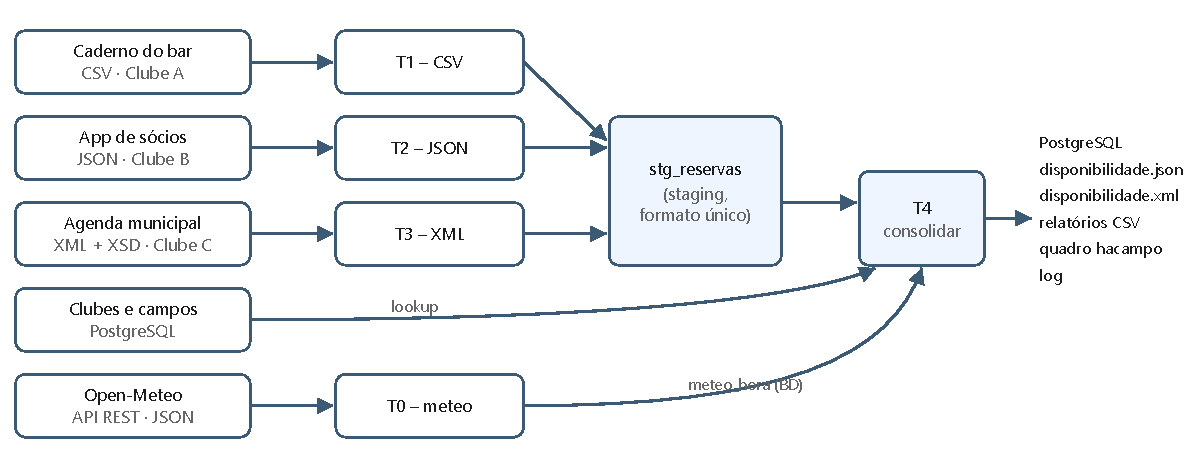
\includegraphics[width=\textwidth]{figuras/arquitetura.pdf}
\caption{Arquitetura do processo: origens, transformações e destinos.}
\label{fig:arquitetura}
\end{figure}

\subsection{Origens (Extract)}

\begin{table}[H]
\centering
\caption{Origens de dados utilizadas.}
\label{tab:origens}
\small
\renewcommand{\arraystretch}{1.2}
\begin{tabular}{@{}p{4.1cm}p{3.1cm}p{2.3cm}p{5cm}@{}}
\toprule
\textbf{Origem} & \textbf{Natureza} & \textbf{Formato} & \textbf{Step do Kettle} \\
\midrule
\texttt{clube\_a\_caderno.csv} & ficheiro local & CSV (\texttt{;}) & \textit{CSV file input} \\
\texttt{clube\_b\_app.json} & ficheiro local & JSON aninhado & \textit{JSON input} (JSONPath) \\
\texttt{clube\_c\_agenda.xml} + \texttt{.xsd} & ficheiro local & XML & \textit{XSD validator} (job) + \textit{Get data from XML} (XPath) \\
tabelas \texttt{clubes} e \texttt{campos} & base de dados relacional & PostgreSQL & \textit{Table input} \\
\texttt{api.open-meteo.com} & serviço web remoto & JSON & \textit{HTTP client} + \textit{JSON input} \\
\bottomrule
\end{tabular}
\end{table}

\subsection{Operadores utilizados (Transform)}

A Tabela~\ref{tab:operadores} relaciona os critérios de mais-valia do enunciado com os operadores utilizados.

\begin{table}[htbp]
\centering
\caption{Critérios do enunciado e operadores correspondentes.}
\label{tab:operadores}
\small
\renewcommand{\arraystretch}{1.25}
\begin{tabular}{@{}p{4.2cm}p{10.6cm}@{}}
\toprule
\textbf{Critério} & \textbf{Onde está no trabalho} \\
\midrule
Expressões regulares & \textit{Replace in string} (normalizar datas, horas, campos e telefones) e \textit{Regex evaluation} (validar e extrair grupos) em T1, T2 e T3 \\
Nulos e validação & \textit{Filter rows} com \texttt{IS NOT NULL} e com os resultados das expressões regulares; linhas inválidas enviadas para ficheiros de erro \\
Duplicados & \textit{Sort rows} + \textit{Unique rows} com redirecionamento dos repetidos (T2 e T4) \\
Anonimização & \textit{Add a checksum} SHA-256 do telefone; \textit{Select values} remove nome, email e telefone \\
Conversão de formatos & CSV, JSON e XML $\rightarrow$ tabela; tabela $\rightarrow$ JSON e XML; datas em texto $\leftrightarrow$ tipo data \\
Junções e \textit{lookups} & \textit{Stream lookup} aos campos e horários e à previsão do tempo \\
Agregações e cálculos & \textit{Calculator} (minutos, duração, n.º de blocos, taxa) e \textit{Group by} (reservas por bloco, ocupação por dia) \\
Reestruturação & \textit{Split fields}, \textit{Value mapper}, \textit{Clone row} (uma reserva $\rightarrow$ $n$ blocos), \textit{String operations}, \textit{Add constants}, \textit{Modified JavaScript value} \\
Orquestração, \textit{logs} e serviços remotos & \textit{job} com tratamento de erros, verificação de ficheiros, validação XSD, SQL, parâmetros, \textit{Write to log} e registo em ficheiro; chamada à API REST \\
\bottomrule
\end{tabular}
\end{table}

\subsection{Destinos (Load)}

Os resultados são carregados no PostgreSQL~\cite{postgres} (esquema \texttt{hacampo}, tabelas \texttt{stg\_reservas}, \texttt{meteo\_hora}, \texttt{ocupacao\_slot} e \texttt{ocupacao\_diaria}), no quadro público \texttt{disponibilidade.json} e \texttt{disponibilidade.xml}, em sete relatórios CSV e no \textit{log} de execução. A página \texttt{src/quadro/index.html} lê o JSON e desenha o quadro livre/ocupado (Figura~\ref{fig:quadro}).

\subsection{Modelo de dados}

A Listagem~\ref{lst:modelo} resume as tabelas criadas pelo \textit{job} (o \textit{script} completo está em \path{src/sql/01_criar_bd.sql}).

\begin{lstlisting}[language={}, caption={Tabelas do esquema \texttt{hacampo}.}, label={lst:modelo}]
clubes          (codigo PK, nome, cidade, latitude, longitude, abertura, fecho, origem)
campos          (clube FK, campo, piso, coberto, iluminacao)               PK (clube, campo)
stg_reservas    (origem, clube, campo, data, inicio_min, fim_min, tipo, cliente_hash, contacto_valido)
meteo_hora      (clube, data_hora, prob_chuva, e_dia)                      PK (clube, data_hora)
ocupacao_slot   (clube, campo, data, hora, nr_reservas, conflito, coberto,
                 prob_chuva, risco_chuva, precisa_luz, sem_luz)            PK (clube, campo, data, hora)
ocupacao_diaria (clube, campo, data, slots_ocupados, slots_totais, taxa_ocupacao)
\end{lstlisting}

As horas são guardadas em \textbf{minutos desde a meia-noite} (18:30 $\rightarrow$ 1110). Desta forma, verificar sobreposições, durações e horários de abertura passa a ser aritmética simples.

% ------------------------------------------------------------------------------
% 4. TRANSFORMAÇÕES
% ------------------------------------------------------------------------------
\newpage
\section{Transformações}

\subsection{T0 -- Previsão do tempo (API REST)}

\begin{figure}[H]
\centering
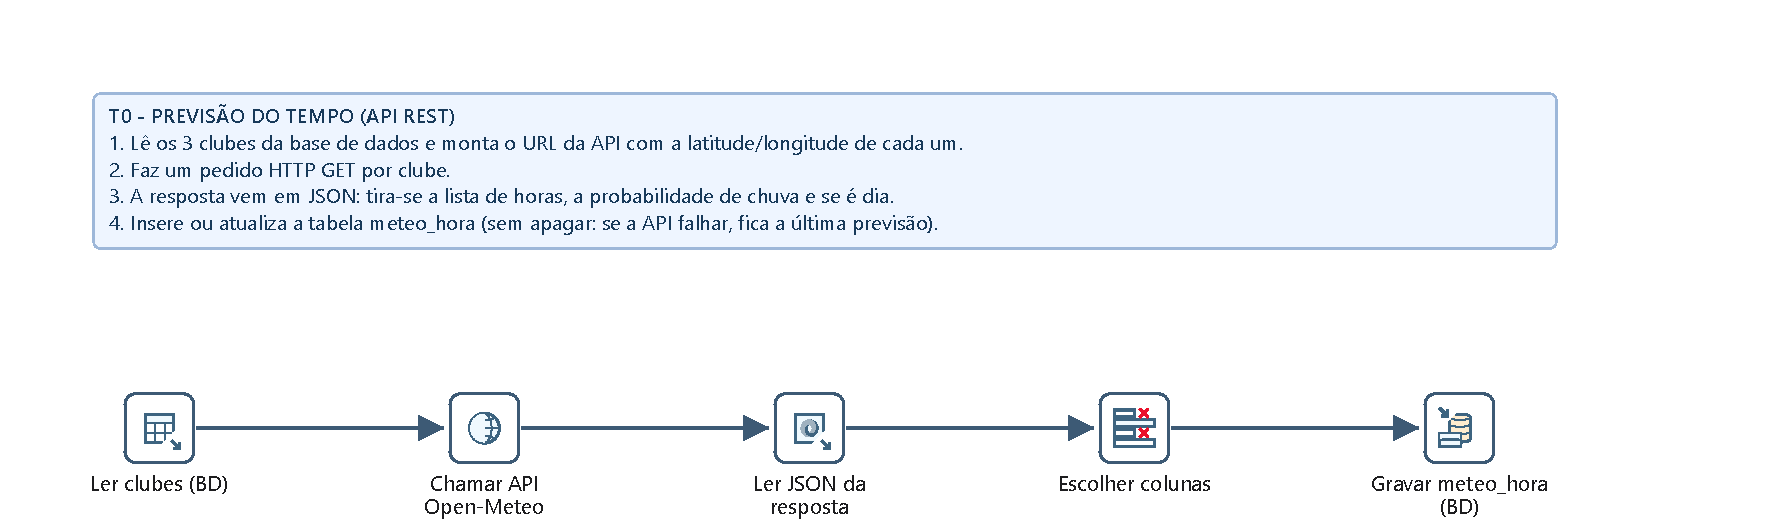
\includegraphics[width=0.85\textwidth]{figuras/t0_meteo_api.pdf}
\caption{Transformação \texttt{t0\_meteo\_api.ktr}.}
\label{fig:t0}
\end{figure}

A transformação lê os três clubes da base de dados e monta, em SQL, o URL da API com a latitude e a longitude de cada um e com os parâmetros \verb!${DATA_INICIO}! e \verb!${DATA_FIM}! (substituição de variáveis ativa). O \textit{HTTP client} faz um pedido GET por clube. A resposta é um JSON com listas paralelas (\texttt{hourly.time}, \texttt{hourly.precipitation\_probability} e \texttt{hourly.is\_day}), que o \textit{JSON input} lê a partir do campo da resposta e transforma em linhas: três pedidos dão 504 linhas (3 clubes $\times$ 7 dias $\times$ 24 horas). O resultado substitui o conteúdo da tabela \texttt{meteo\_hora}.

\subsection{T1 -- Clube A: caderno do bar (CSV)}

\begin{figure}[H]
\centering
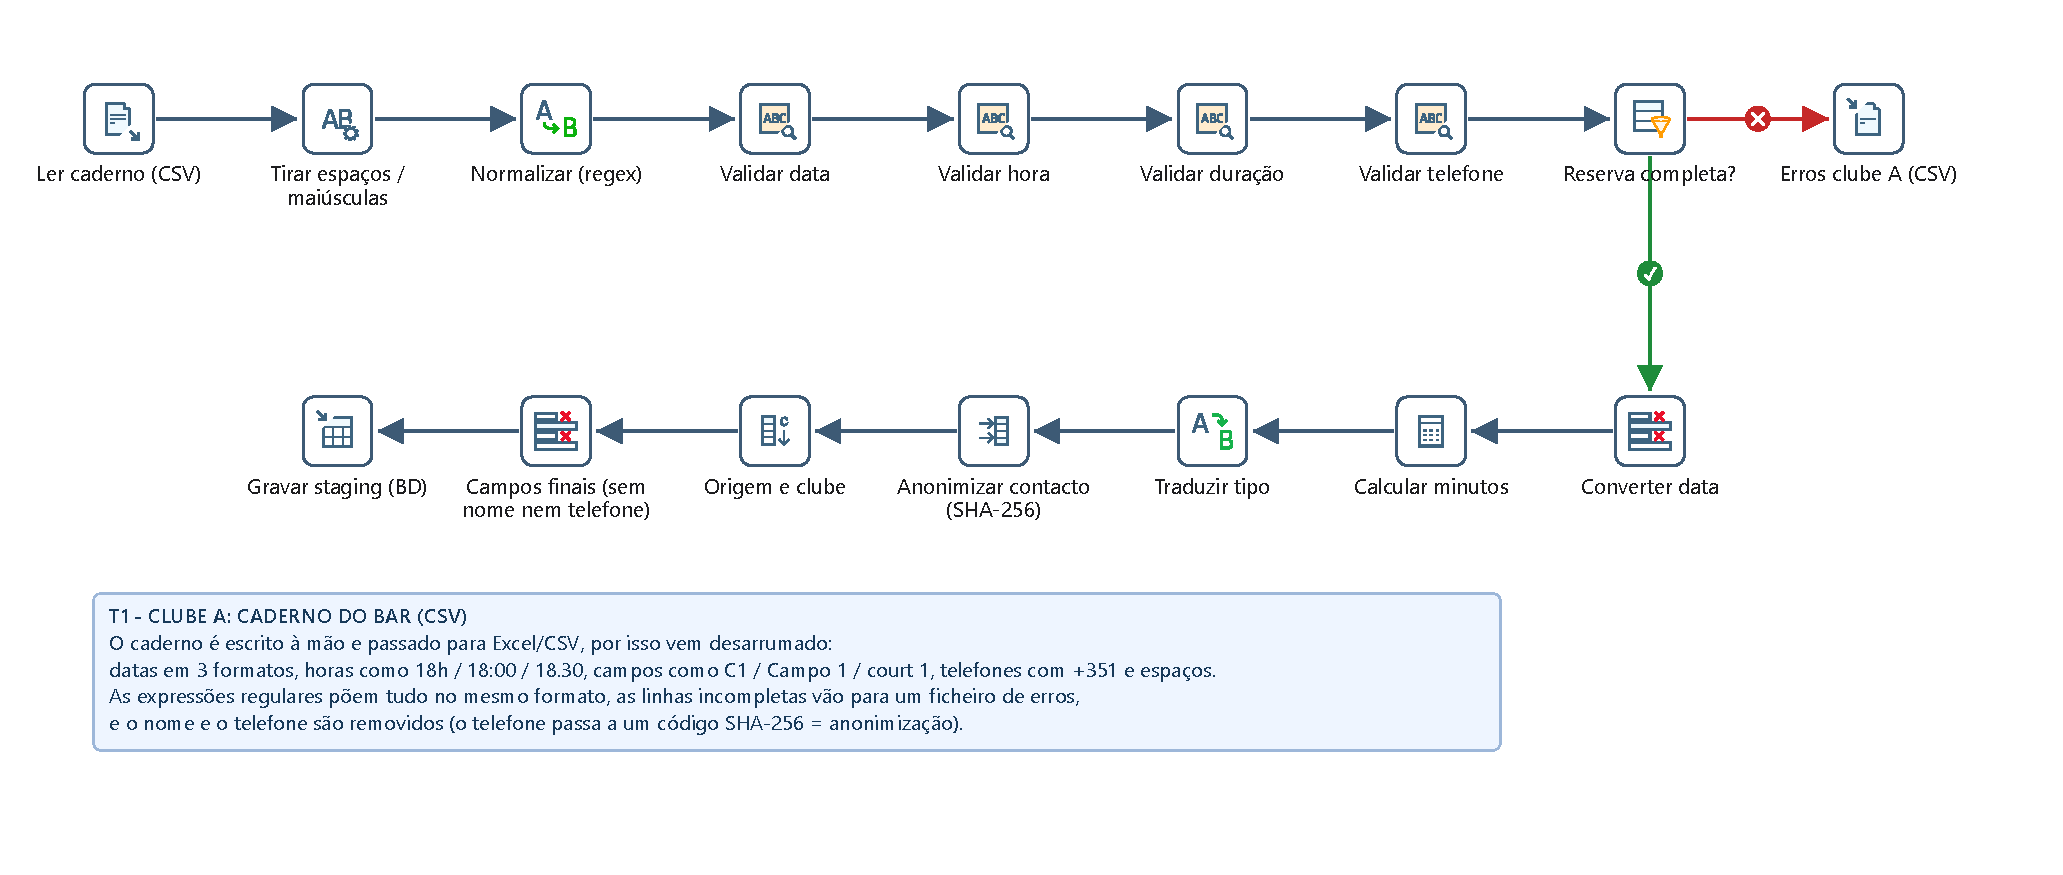
\includegraphics[width=\textwidth]{figuras/t1_clube_a_csv.pdf}
\caption{Transformação \texttt{t1\_clube\_a\_csv.ktr}.}
\label{fig:t1}
\end{figure}

É a origem mais desorganizada. Primeiro, o \textit{String operations} retira espaços, coloca a hora e o tipo em maiúsculas e o nome com iniciais maiúsculas. Depois, o \textit{Replace in string} aplica as expressões regulares~\cite{regex} da Tabela~\ref{tab:regex}.

\begin{table}[H]
\centering
\caption{Expressões regulares de normalização (T1).}
\label{tab:regex}
\small
\renewcommand{\arraystretch}{1.25}
\begin{tabular}{@{}p{1.5cm}p{5.4cm}p{2.2cm}p{5.4cm}@{}}
\toprule
\textbf{Campo} & \textbf{Expressão regular} & \textbf{Substituição} & \textbf{Exemplo} \\
\midrule
data & \verb!^(\d{2})/(\d{2})/(\d{4})$! & \verb!$3-$2-$1! & \texttt{21/10/2026} $\rightarrow$ \texttt{2026-10-21} \\
data & \verb!^(\d{2})-(\d{2})-(\d{2})$! & \verb!20$3-$2-$1! & \texttt{21-10-26} $\rightarrow$ \texttt{2026-10-21} \\
hora & \verb!^(\d{1,2})[H:.]?$! & \verb!$1:00! & \texttt{18H} $\rightarrow$ \texttt{18:00} \\
hora & \verb!^(\d{1,2})[H:.](\d{2})$! & \verb!$1:$2! & \texttt{18h30}, \texttt{18.30} $\rightarrow$ \texttt{18:30} \\
campo & \verb!\D! & (vazio) & \texttt{Campo 2}, \texttt{C2}, \texttt{court 2} $\rightarrow$ \texttt{2} \\
telefone & \verb!\D! e depois \verb!^(00351|351)(\d{9})$! & \verb!$2! & \texttt{+351 912 345 678} $\rightarrow$ \texttt{912345678} \\
\bottomrule
\end{tabular}
\end{table}

A seguir, quatro passos \textit{Regex evaluation} validam os valores já normalizados e, através dos grupos de captura, extraem os números de que o cálculo precisa:
\begin{itemize}[itemsep=1pt]
    \item data: \verb!^\d{4}-\d{2}-\d{2}$!;
    \item hora: \verb!^(\d{1,2}):(\d{2})$! $\rightarrow$ \texttt{h\_ini}, \texttt{m\_ini};
    \item duração: \verb!^(?:(\d+)\s*h)?\s*(?:(\d+)\s*(?:min|m)?)?$!, que aceita \texttt{1h}, \texttt{1h30}, \texttt{90min} e \texttt{60} $\rightarrow$ \texttt{dur\_h}, \texttt{dur\_m};
    \item telefone português: \verb!^(9[1236]\d{7}|2\d{8})$!.
\end{itemize}

O \textit{Filter rows} envia as linhas incompletas para \texttt{erros\_clube\_a.csv}. As restantes seguem: a data passa a tipo data, o \textit{Calculator} calcula $\mathit{inicio\_min} = h \times 60 + m$ e $\mathit{fim\_min} = \mathit{inicio\_min} + \mathit{duração}$ (com \texttt{NVL} para as partes em falta), o \textit{Value mapper} traduz S/P/A para singulares/pares/aula e o \textit{Add a checksum} substitui o telefone por um código SHA-256. Este código permite contar clientes e detetar duplicados sem guardar o número (pseudonimização, no sentido do RGPD~\cite{rgpd}). O último \textit{Select values} deixa apenas os campos da \textit{staging}: o nome e o telefone ficam para trás.

\textbf{Resultado:} 48 linhas lidas, 2 com erro (uma sem hora e outra com a data sem ano) e 46 gravadas na \textit{staging}.

\subsection{T2 -- Clube B: aplicação de sócios (JSON)}

\begin{figure}[H]
\centering
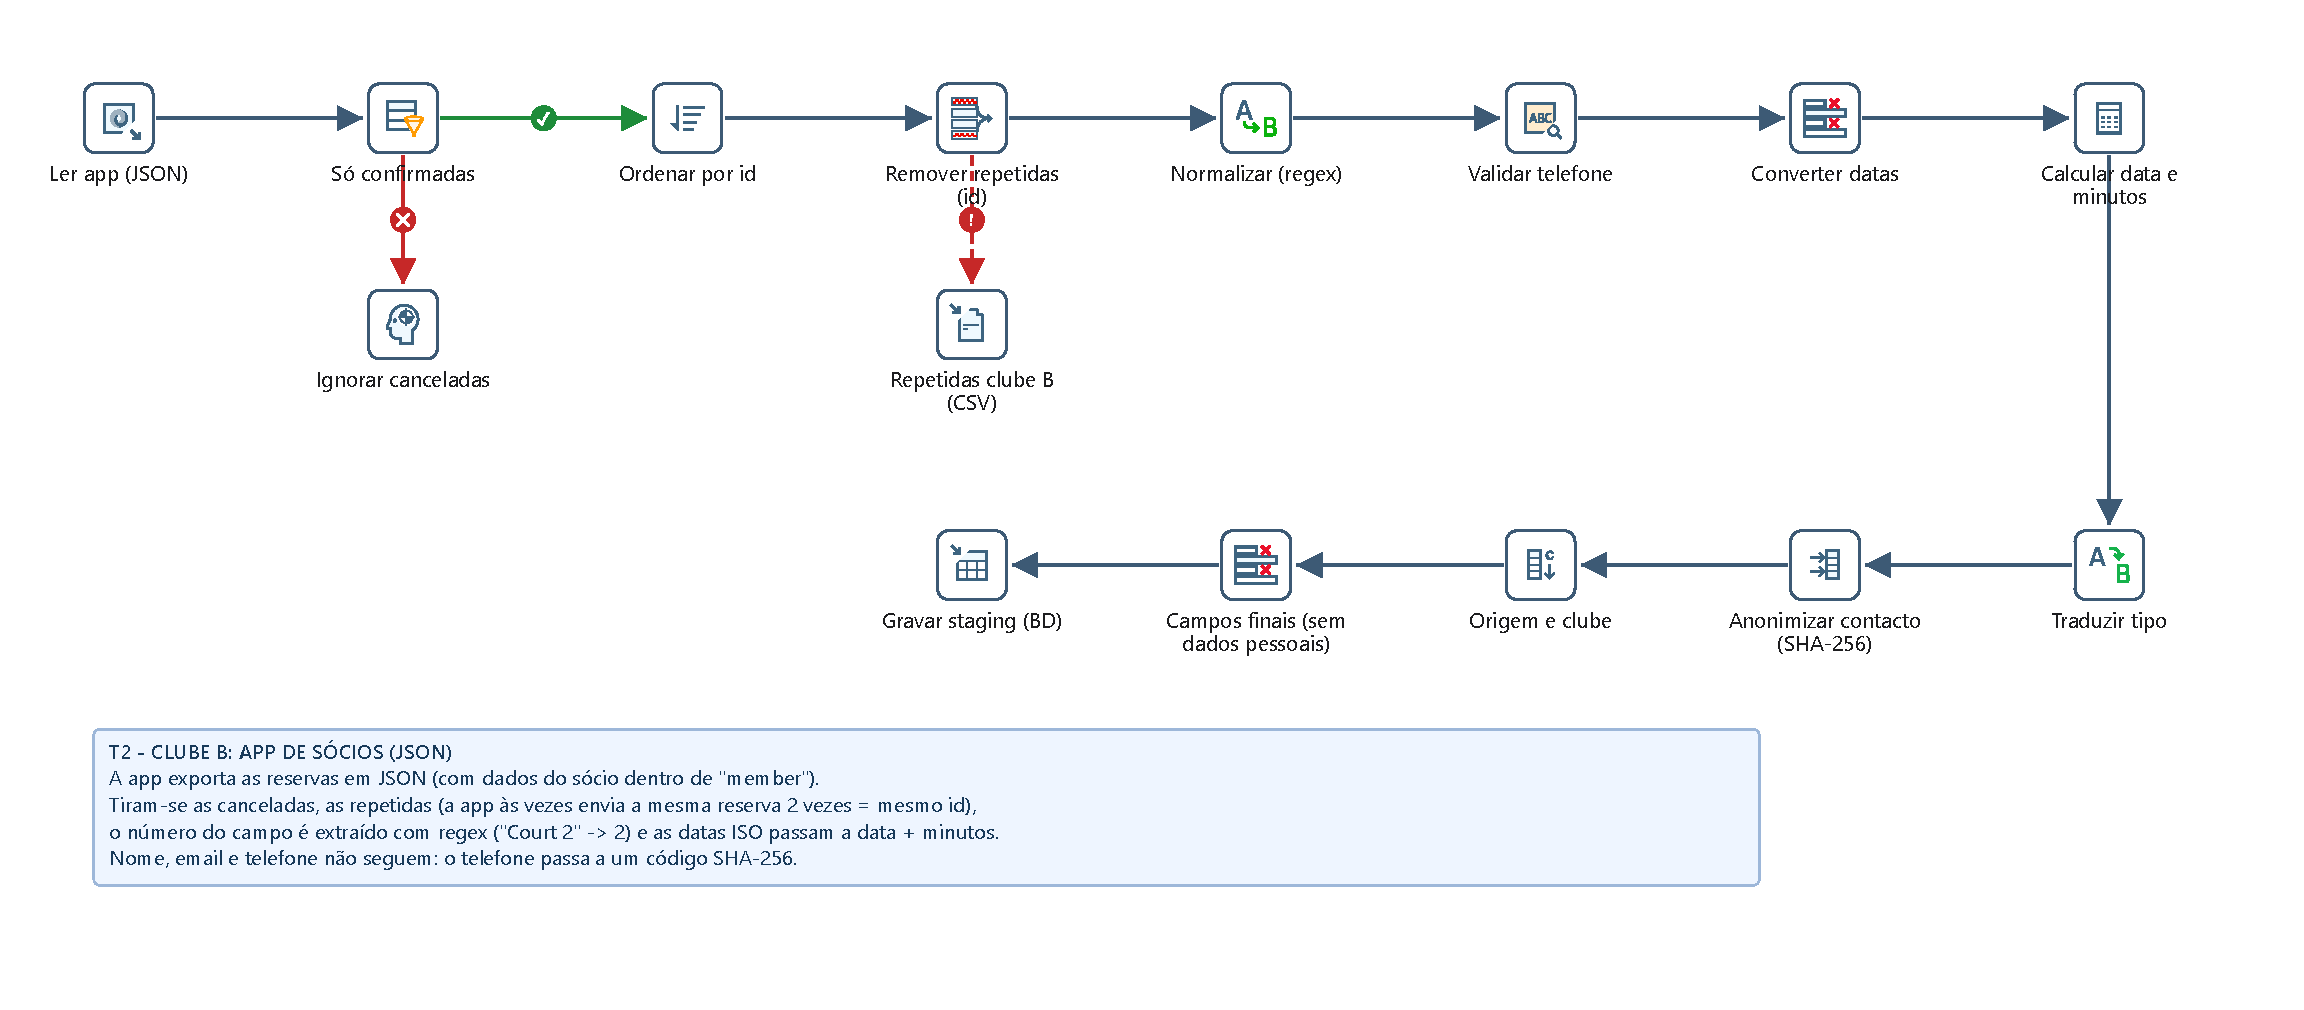
\includegraphics[width=\textwidth]{figuras/t2_clube_b_json.pdf}
\caption{Transformação \texttt{t2\_clube\_b\_json.ktr}.}
\label{fig:t2}
\end{figure}

O \textit{JSON input} usa caminhos JSONPath como \verb!$.reservas[*].member.phone! para achatar o objeto aninhado do sócio. As reservas com \texttt{status} diferente de \texttt{confirmed} são descartadas. Depois de ordenar por \texttt{id}, o \textit{Unique rows} deteta os registos que a aplicação enviou duas vezes e redireciona-os, através de um \textit{hop} de erro, para \texttt{repetidas\_clube\_b.csv}. As datas ISO (\texttt{2026-10-21T18:00:00}) são convertidas para o tipo data e o \textit{Calculator} extrai a data sem hora (\texttt{REMOVE\_TIME\_FROM\_DATE}), a hora (\texttt{HOUR\_OF\_DAY}) e o minuto (\texttt{MINUTE\_OF\_HOUR}). O nome, o email e o telefone não passam para a \textit{staging}.

\textbf{Resultado:} 51 reservas lidas, 7 canceladas, 2 repetidas e 42 gravadas.

\subsection{T3 -- Clube C: agenda municipal (XML)}

\begin{figure}[H]
\centering
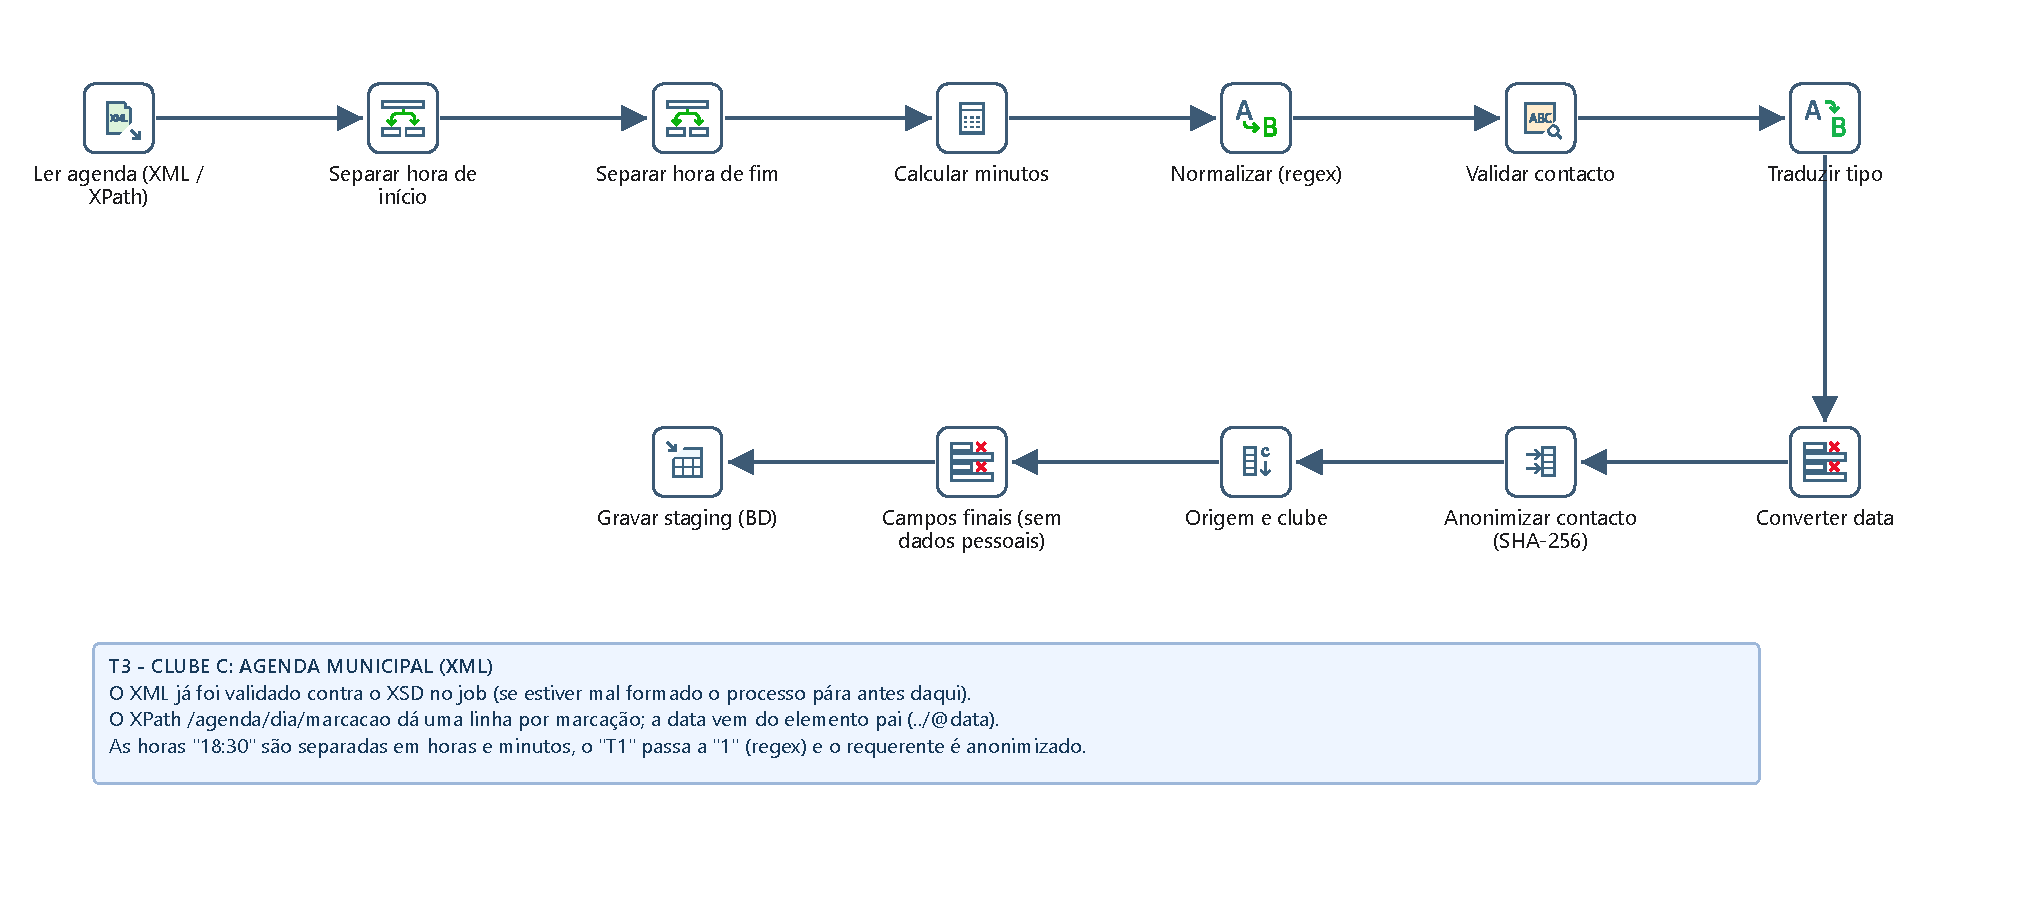
\includegraphics[width=0.95\textwidth]{figuras/t3_clube_c_xml.pdf}
\caption{Transformação \texttt{t3\_clube\_c\_xml.ktr}.}
\label{fig:t3}
\end{figure}

Antes desta transformação, o \textit{job} valida o XML contra \texttt{clube\_c\_agenda.xsd}~\cite{xsd}. O XSD obriga, por exemplo, a horas no formato \texttt{HH:MM}, a campos \texttt{T1}, \texttt{T2}, \ldots{} e a um tipo de marcação dentro de uma lista fechada; se o XML não cumprir estas regras, o processo pára antes de ler dados errados. O \textit{Get data from XML} percorre \texttt{/agenda/dia/marcacao} (uma linha por marcação) e obtém a data a partir do elemento pai com o XPath \texttt{../@data}. As horas \texttt{18:30} são separadas com \textit{Split fields}, o código \texttt{T1} passa a \texttt{1} com a expressão regular \verb!^T! e o requerente é anonimizado.

\textbf{Resultado:} 32 marcações gravadas.

\subsection{T4 -- Consolidar e publicar}

\begin{figure}[H]
\centering
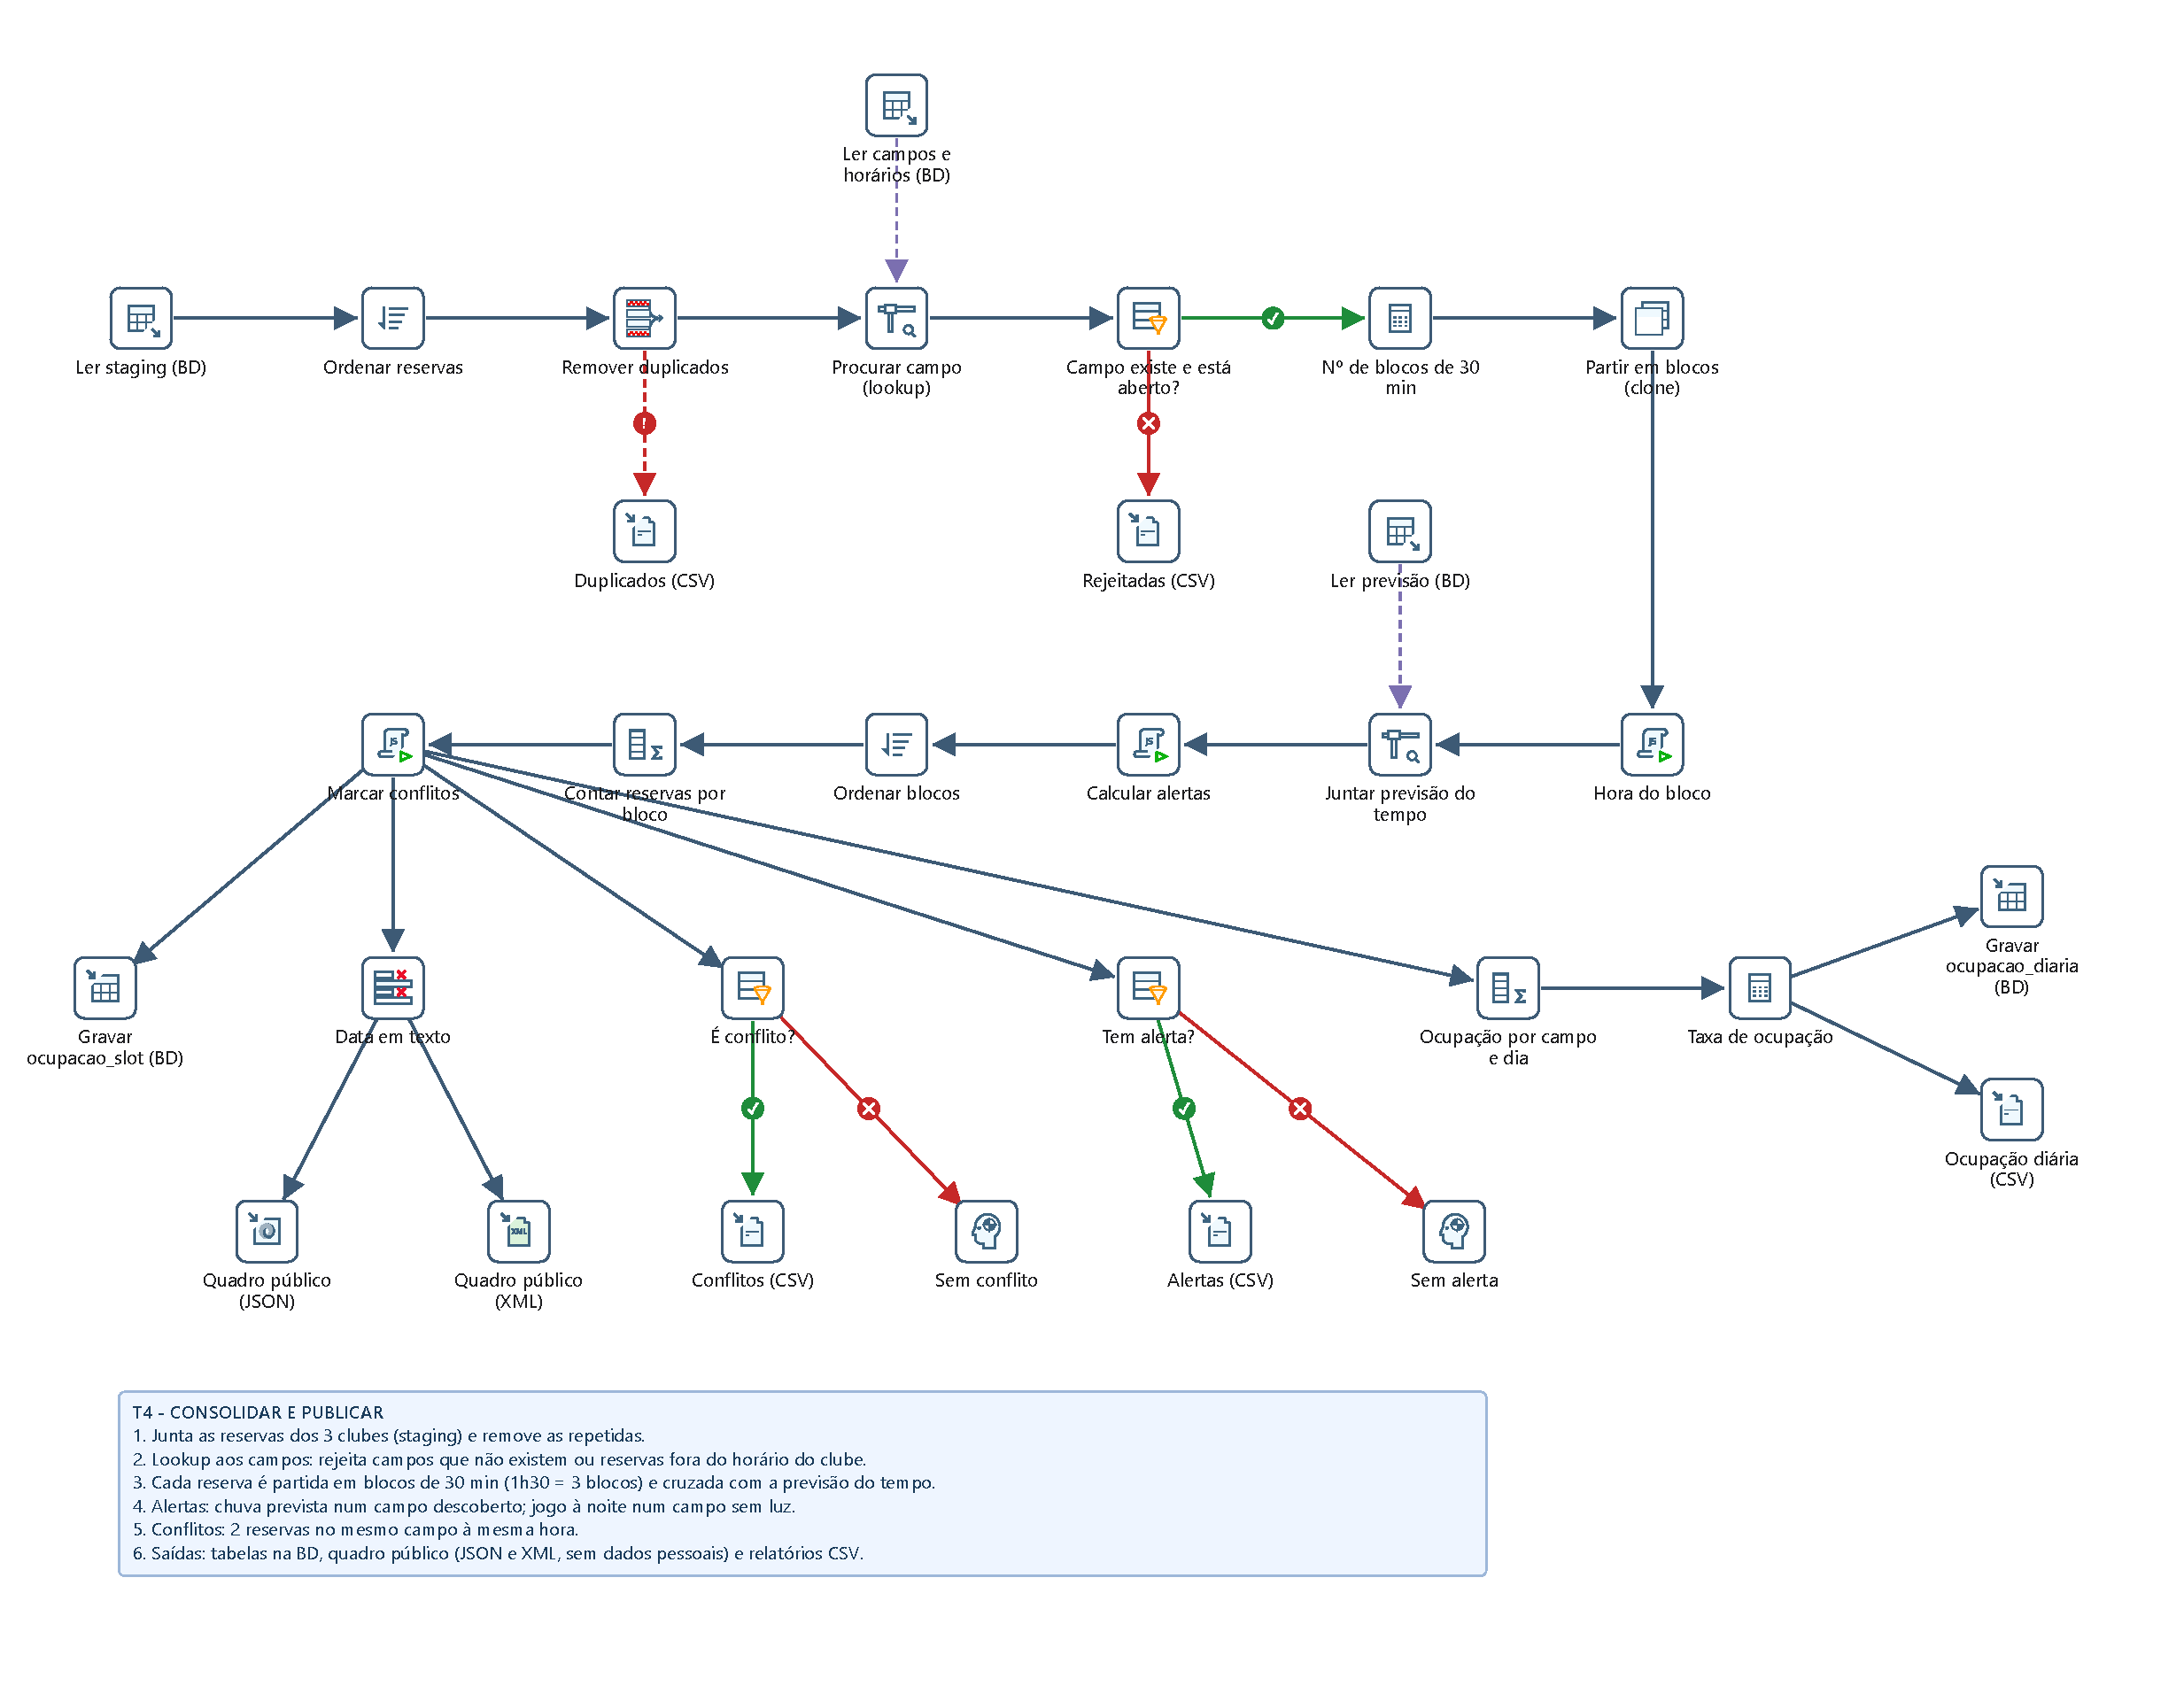
\includegraphics[width=0.92\textwidth]{figuras/t4_consolidar_publicar.pdf}
\caption{Transformação \texttt{t4\_consolidar\_publicar.ktr}.}
\label{fig:t4}
\end{figure}

A transformação T4 junta as reservas dos três clubes e aplica as regras de negócio:
\begin{enumerate}[itemsep=2pt]
    \item \textbf{Duplicados:} lê a \textit{staging}, ordena e remove a mesma reserva escrita duas vezes (mesmo clube, campo, data, horas e cliente), que segue para \texttt{duplicados.csv}.
    \item \textbf{Validação de negócio:} um \textit{Stream lookup} a \texttt{campos} + \texttt{clubes} acrescenta se o campo é coberto, se tem iluminação e o horário em minutos. O \textit{Filter rows} compara campos entre si ($\mathit{inicio\_min} \geq \mathit{abertura\_min}$ e $\mathit{fim\_min} \leq \mathit{fecho\_min}$) e rejeita campos inexistentes e reservas fora do horário para \texttt{rejeitadas.csv}.
    \item \textbf{Blocos de 30 minutos:} o \textit{Calculator} calcula o número de blocos (1h30 $\rightarrow$ 3) e o \textit{Clone row} cria uma cópia por bloco, numerada. O passo \textit{Hora do bloco} (Listagem~\ref{lst:hora}) calcula a hora de cada bloco e a chave da meteorologia.
    \item \textbf{Meteorologia:} um \textit{Stream lookup} a \texttt{meteo\_hora} por clube e hora permite calcular os alertas (Listagem~\ref{lst:alertas}): \texttt{risco\_chuva} (campo descoberto e probabilidade $\geq$ \texttt{LIMITE\_CHUVA}), \texttt{precisa\_luz} (já é noite) e \texttt{sem\_luz} (é noite e o campo não tem iluminação).
    \item \textbf{Conflitos:} o \textit{Group by} conta as reservas por campo, dia e bloco; mais de uma reserva no mesmo bloco é um conflito, que segue para \texttt{conflitos.csv}.
    \item \textbf{Saídas:} as linhas são copiadas em paralelo para a tabela \texttt{ocupacao\_slot}, para o quadro em JSON e em XML, para os ficheiros de alertas e de conflitos e, com um segundo \textit{Group by} e um \textit{Calculator}, para a taxa de ocupação por campo e por dia (base de dados e CSV).
\end{enumerate}

\begin{lstlisting}[language=Java, caption={Passo \textit{Hora do bloco} (Modified JavaScript value).}, label={lst:hora}]
// cada cópia da reserva corresponde a um bloco de 30 minutos
var minuto = inicio_min + bloco * 30;
var hh = Math.floor(minuto / 60);
var mm = minuto % 60;
function dois(n) { return (n < 10 ? "0" : "") + n; }
var hora = dois(hh) + ":" + dois(mm);
// chave igual à da API: 2026-10-21T18:00
var chave_meteo = date2str(data, "yyyy-MM-dd") + "T" + dois(hh) + ":00";
\end{lstlisting}

\begin{lstlisting}[language=Java, caption={Passo \textit{Calcular alertas} (Modified JavaScript value).}, label={lst:alertas}]
// os campos booleanos vêm da BD como objetos Java: compara-se com true/false
var descoberto = (coberto == false);
var tem_luz = (iluminacao == true);
// a chuva só interessa nos campos descobertos (limite em %: parâmetro LIMITE_CHUVA)
var limite = parseInt(getVariable("LIMITE_CHUVA", "50"));
var risco_chuva = (descoberto && prob_chuva != null && prob_chuva >= limite);
// e_dia = 0 -> já é noite, o campo precisa de luz
var precisa_luz = (e_dia != null && e_dia == 0);
var sem_luz = (precisa_luz && !tem_luz);
\end{lstlisting}

A Tabela~\ref{tab:resultados} resume uma execução completa do processo.

\begin{table}[H]
\centering
\caption{Resultados da execução de 20 de outubro de 2026.}
\label{tab:resultados}
\small
\renewcommand{\arraystretch}{1.2}
\begin{tabular}{@{}p{10cm}p{4.8cm}@{}}
\toprule
\textbf{Indicador} & \textbf{Valor} \\
\midrule
Reservas na \textit{staging} (3 clubes) & 120 \\
Duplicados removidos / rejeitadas (campo inexistente, fora de horas) & 2 / 2 \\
Reservas válidas $\rightarrow$ blocos de 30 minutos & 116 $\rightarrow$ 316 \\
Blocos ocupados distintos / em conflito & 311 / 5 \\
Blocos com alerta (noite num campo sem luz) & 14 \\
Blocos com chuva $\geq$ 50\% num campo descoberto & 0 (semana seca; com \texttt{LIMITE\_CHUVA = 5} há 99) \\
Linhas de ocupação diária (campo $\times$ dia) & 60 \\
\bottomrule
\end{tabular}
\end{table}

% ------------------------------------------------------------------------------
% 5. JOBS
% ------------------------------------------------------------------------------
\newpage
\section{Jobs}

\begin{figure}[H]
\centering
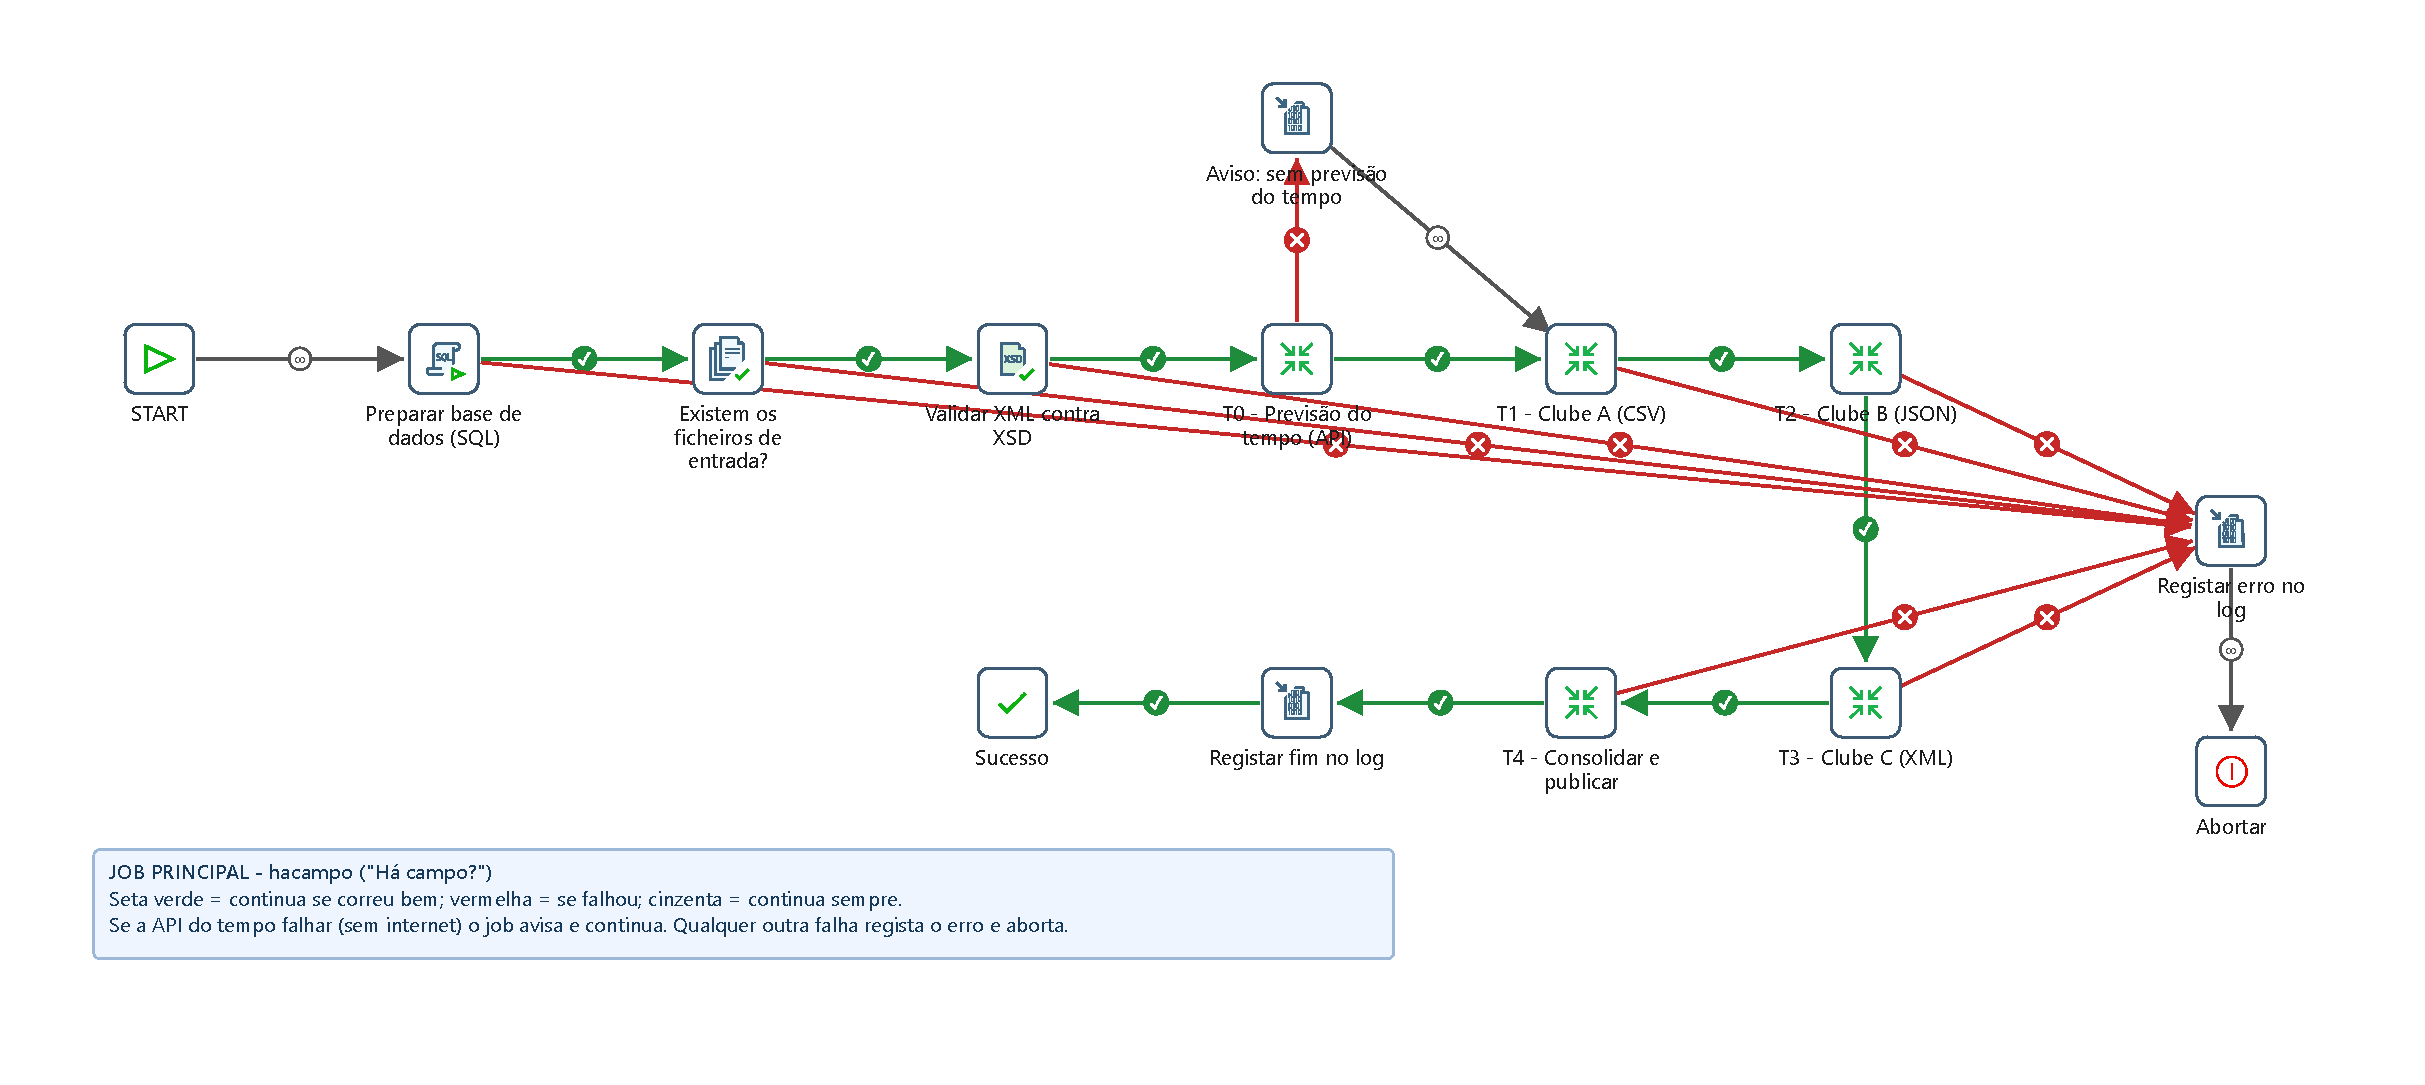
\includegraphics[width=\textwidth]{figuras/j_hacampo.pdf}
\caption{\textit{Job} principal \texttt{j\_hacampo.kjb}.}
\label{fig:job}
\end{figure}

O \textit{job} \texttt{j\_hacampo.kjb} (Figura~\ref{fig:job}) define a ordem de execução e o que acontece quando algum passo falha:
\begin{enumerate}[itemsep=2pt]
    \item \textbf{Preparar base de dados (SQL):} cria o esquema e as tabelas se não existirem, insere ou atualiza os clubes e os campos (\texttt{INSERT \ldots{} ON CONFLICT \ldots{} DO UPDATE}) e esvazia a \textit{staging}. Pode ser executado várias vezes.
    \item \textbf{Existem os ficheiros de entrada?} Verifica que os três ficheiros existem.
    \item \textbf{Validar XML contra XSD.}
    \item \textbf{T0 -- Previsão do tempo.} Se falhar (por exemplo, sem ligação à Internet), escreve um aviso no \textit{log} e continua com a última previsão guardada; é o único passo que pode falhar sem interromper o processo.
    \item \textbf{T1, T2 e T3} carregam a \textit{staging}; \textbf{T4} consolida e publica.
    \item \textbf{Fim:} regista no \textit{log} onde estão os resultados e termina com \textit{Success}. Qualquer falha nos passos 1 a 3 ou em T1 a T4 segue o \textit{hop} vermelho: o erro é registado no \textit{log} e o \textit{job} é abortado.
\end{enumerate}

O \textit{job} tem três parâmetros, passados às transformações: \texttt{DATA\_INICIO} e \texttt{DATA\_FIM} (semana pedida à API) e \texttt{LIMITE\_CHUVA}. Todos os caminhos são relativos à pasta dos ficheiros (variável \path{${Internal.Entry.Current.Directory}}), pelo que a pasta pode ser copiada para outro computador. A Listagem~\ref{lst:kitchen} mostra a execução pela linha de comandos.

\begin{lstlisting}[language={}, caption={Execução do \textit{job} com o Kitchen, com registo em ficheiro.}, label={lst:kitchen}]
Kitchen.bat -file="...\dataintegration\j_hacampo.kjb" -level=Basic "-logfile=...\data\output\execucao.log"
\end{lstlisting}

A Figura~\ref{fig:quadro} mostra o resultado final: o quadro \textit{``Há campo?''} a ler o ficheiro \texttt{disponibilidade.json} produzido pela T4.

\begin{figure}[H]
\centering
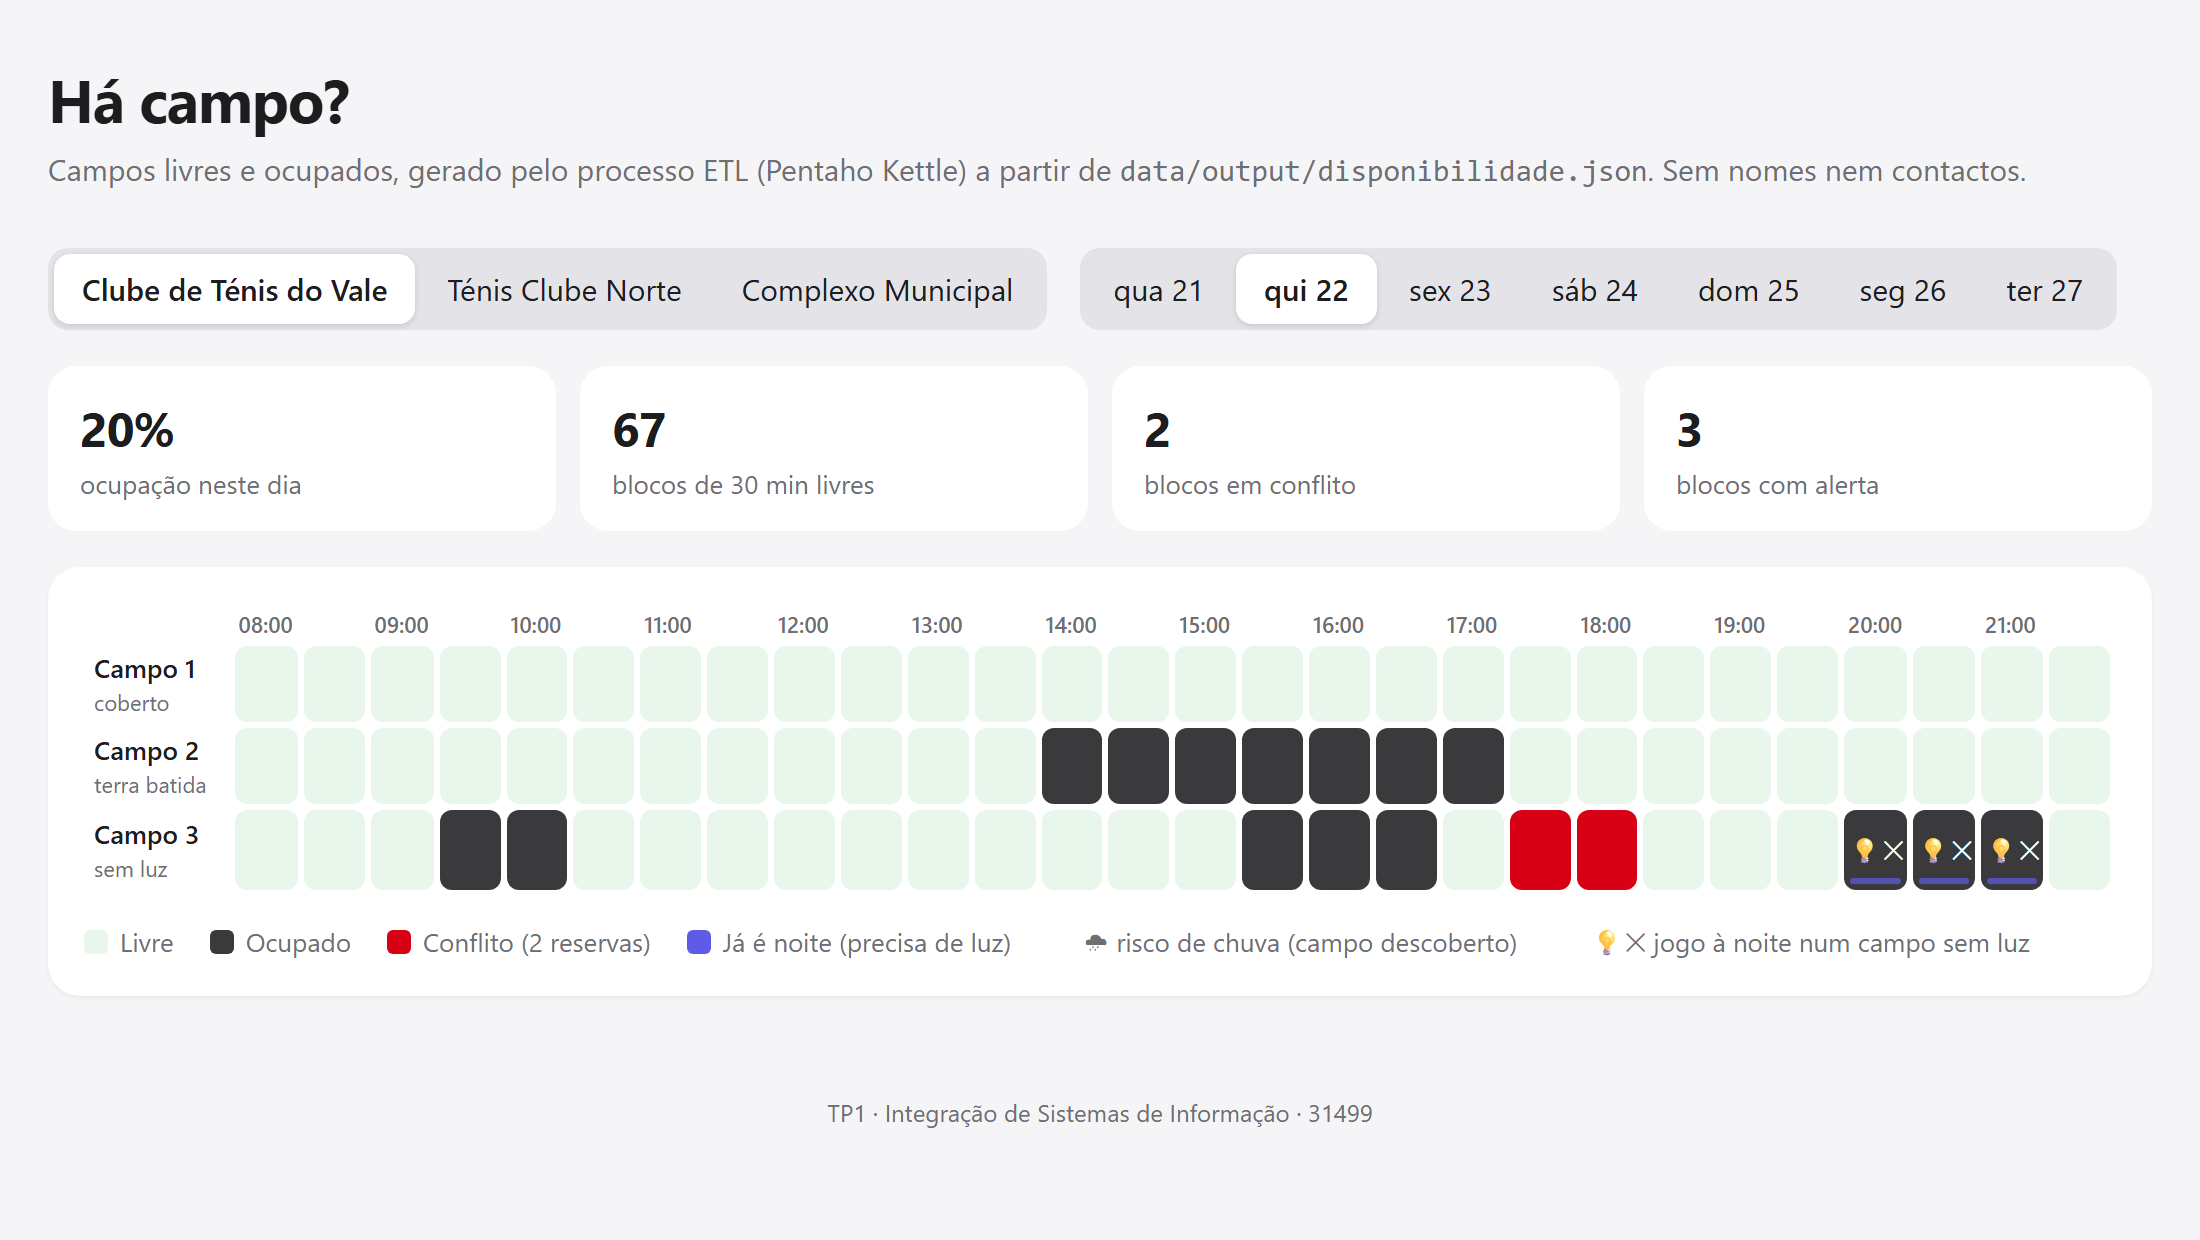
\includegraphics[width=\textwidth]{figuras/quadro.png}
\caption{Quadro \textit{``Há campo?''} (\texttt{src/quadro/index.html}): ocupado a cinzento, conflito a vermelho, jogo à noite num campo sem luz assinalado.}
\label{fig:quadro}
\end{figure}

% ------------------------------------------------------------------------------
% 6. VÍDEO
% ------------------------------------------------------------------------------
\section{Vídeo com demonstração}

O vídeo mostra a execução do \textit{job} no Spoon, os dados de entrada com erros, os ficheiros de saída, as tabelas no PostgreSQL e o quadro final.

\begin{videoBox}{Vídeo de demonstração}
\ifx\videoURL\empty
    {\color{red}\textit{ligação ao vídeo por inserir}}
\else
    \begin{minipage}[c]{3.3cm}
        \begingroup\edef\x{\endgroup\noexpand\qrcode[height=3cm]{\videoURL}}\x
    \end{minipage}%
    \hfill
    \begin{minipage}[c]{0.72\linewidth}
        \textbf{Demonstração do processo ETL \textit{``Há campo?''}}\\[2pt]
        \expandafter\url\expandafter{\videoURL}
    \end{minipage}
\fi
\end{videoBox}

% ------------------------------------------------------------------------------
% 7. CONCLUSÃO
% ------------------------------------------------------------------------------
\section{Conclusão e trabalhos futuros}

O trabalho apresenta um processo ETL completo sobre um problema real: juntar num único quadro as marcações de clubes que utilizam sistemas diferentes. O processo lê cinco origens (CSV, JSON, XML, PostgreSQL e uma API REST); limpa e normaliza os dados com expressões regulares; remove repetidos; anonimiza os dados pessoais; e aplica regras de negócio (horários, campos existentes, conflitos, luz e chuva). Os resultados ficam na base de dados e em ficheiros JSON, XML e CSV. A separação entre transformações de entrada, \textit{staging} e consolidação facilita a integração de novos clubes.

As principais dificuldades foram as datas e horas escritas de muitas formas diferentes, a decisão sobre o que é um erro (enviado para ficheiro) e o que é apenas um aviso (a linha continua), e a anonimização sem perder a capacidade de detetar duplicados, resolvida com o código SHA-256 do contacto.

Como trabalhos futuros, propõe-se:
\begin{itemize}[itemsep=1pt]
    \item executar o \textit{job} de hora a hora (agendador do sistema ou Carte) e publicar o JSON automaticamente no site hacampo (FTP/SFTP);
    \item enviar por email ao clube os conflitos e alertas do dia (entrada \textit{Mail} do \textit{job});
    \item receber as marcações em tempo real por MQTT/Node-RED, em vez de ficheiros;
    \item ligar o processo a clubes reais, com a respetiva autorização.
\end{itemize}

% ------------------------------------------------------------------------------
% 8. REFERÊNCIAS
% ------------------------------------------------------------------------------
\section{Referências}
\begingroup
\renewcommand{\section}[2]{}
\begin{thebibliography}{99}
\bibitem{enunciado}
Instituto Politécnico do Cávado e do Ave, \emph{Integração de Sistemas de Informação -- Trabalho Prático I}, enunciado, 2026/27. Material disponibilizado na unidade curricular.

\bibitem{slides}
Instituto Politécnico do Cávado e do Ave, \emph{Integração de Sistemas de Informação -- slides das aulas} (Integração ao nível dos dados: XML e XML em C\#; ETL: introdução, \textit{Kettle Tutorial} e acesso a bases de dados), 2026/27. Material disponibilizado na unidade curricular.

\bibitem{casters}
M. Casters, R. Bouman e J. van Dongen, \emph{Pentaho Kettle Solutions: Building Open Source ETL Solutions with Pentaho Data Integration}. Indianapolis: Wiley, 2010.

\bibitem{pdi}
Pentaho, \emph{Pentaho Data Integration -- documentação de \textit{steps} e \textit{job entries}}, \url{https://pentaho-public.atlassian.net/wiki/spaces/EAI}. Consultado em 20 de outubro de 2026.

\bibitem{openmeteo}
Open-Meteo, \emph{Weather Forecast API} (parâmetros \texttt{hourly}, \texttt{precipitation\_probability} e \texttt{is\_day}), \url{https://open-meteo.com/en/docs}. Consultado em 20 de outubro de 2026.

\bibitem{postgres}
The PostgreSQL Global Development Group, \emph{PostgreSQL 17 Documentation} (\texttt{INSERT \ldots{} ON CONFLICT}, \texttt{CREATE TABLE IF NOT EXISTS}), \url{https://www.postgresql.org/docs/17/}. Consultado em 20 de outubro de 2026.

\bibitem{xsd}
W3C, \emph{XML Schema Part 2: Datatypes} (\texttt{xs:pattern}, \texttt{xs:enumeration}), \url{https://www.w3.org/TR/xmlschema-2/}. Consultado em 20 de outubro de 2026.

\bibitem{regex}
J. Goyvaerts e S. Levithan, \emph{Regular Expressions Cookbook}. Sebastopol: O'Reilly Media, 2009.

\bibitem{rgpd}
Regulamento (UE) 2016/679 do Parlamento Europeu e do Conselho (Regulamento Geral sobre a Proteção de Dados), artigos 4.º e 25.º.
\end{thebibliography}
\endgroup

% ------------------------------------------------------------------------------
% ANEXO A
% ------------------------------------------------------------------------------
\section*{Anexo A -- Declaração de utilização de inteligência artificial}
\addcontentsline{toc}{section}{Anexo A -- Declaração de utilização de inteligência artificial}

Foi utilizado um assistente de IA (modelo de linguagem) na análise do enunciado, no desenvolvimento do processo ETL e na redação do relatório, a partir de pedidos de escolha do tema, planeamento e execução do trabalho e organização da entrega.

\end{document}
